\begin{center}
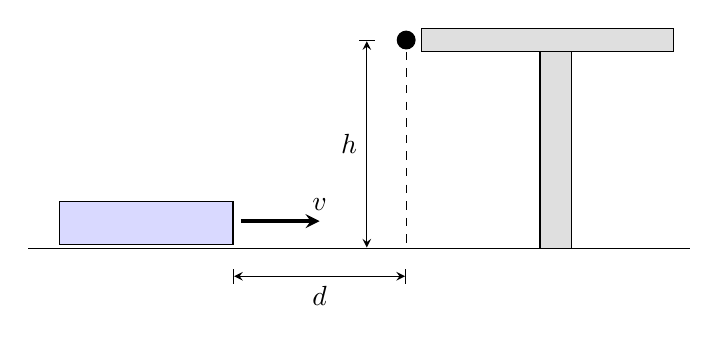
\begin{tikzpicture}[>=stealth]
 \draw (-5,0) -- (3.4,0);
 \fill[gray!25] (0,2.5) rectangle (3.2,2.8);
 \draw (0,2.5) rectangle (3.2,2.8);
 \fill[gray!25] (1.5,0) rectangle (1.9,2.5);
 \draw (1.5,0) rectangle (1.9,2.5);
 \fill (-0.2,2.65) circle (0.12);
 \draw[dashed] (-0.2,2.5) -- (-0.2,0.05);
 \draw[|<->|] (-0.7,0) -- (-0.7,2.65) node[midway, left] {$h$};
 \draw[fill=blue!15] (-4.6,0.05) rectangle (-2.4,0.6);
 \draw[->, very thick] (-2.3,0.35) -- (-1.3,0.35) node[above] {$v$};
 \draw[|<->|] (-2.4,-0.35) -- (-0.2,-0.35) node[midway, below] {$d$};
\end{tikzpicture}
\end{center}

Der Stuntman fällt die Höhe $h$ in der Zeit
\begin{align}
 h &= \frac{1}{2}g\,t^2 \quad\Rightarrow\quad t = \sqrt{\frac{2h}{g}}
\end{align}
In dieser Zeit muss der Zug mit der Geschwindigkeit $v$ die Strecke $d$ bis unter die Brücke zurücklegen:
\begin{align}
 d &= v\,t = \dzF \\
   &= \vz\cdot\sqrt{\frac{2\cdot\hbr}{\gE}} \\
   &= \dz \approx \result{\dzP{0}{2}}
\end{align}
Die Höhe des Zuges ist vernachlässigt; sie verkürzt die Fallhöhe und damit $d$.
